\chapter{Manual Annotation} \label{chapter:manual_annotation}

\begin{figure}[!tbp]
	\centering
    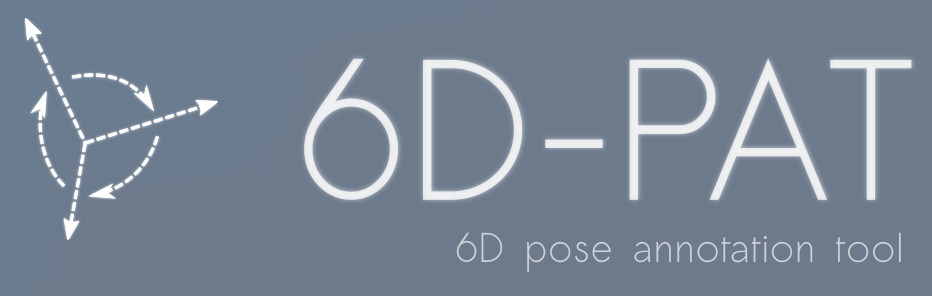
\includegraphics[width=\linewidth]{6dpat}
    \caption{The logo of the pose annotation tool 6D-PAT. Own image.}
    	\label{fig:6dpat_logo}
\end{figure} 

The following chapter analyzes manual 6D pose annotation process and its prerequisites. To this end, the necessary terminology is defined and explained and the workflow to annotate poses using the developed annotation tool is described. The assessment of the requirements of the annotation procedure and the creation of the tool are conducted based on the medical image dataset, which is described further below.

\section{Terminology} \label{section:terminology}

\textbf{Image.} An image $I$ is a 2D matrix of pixels. The pixel $u$ at position $(i, j)$ is referenced by the tuple $(x, y)$, where $x = j$ and $y = i$. The inverted notation is chosen over the common row-major matrix indexing to account for the universal  \\

\noindent\textbf{Object Model.} An \textit{object model}, or \textit{3D model}, $O$ is composed of a set of points $M \subseteq \mathbb{R}^3$ and a set of triangles $T = \{(m_1, m_2, m_3) \in M^3\}$, also called mesh. The real-world entity that the object model resembles is not restricted. In case of the T-Less dataset \cite{tless} the objects are mainly hardware like screws and power sockets. \\

\noindent\textbf{6D Pose.} A \textit{6D pose} $P$ is the tuple $(R, t)$, where $R$ is the 3x3 rotation matrix and $t$ the translation vector used to transform the respective object model into camera coordinates (see section \ref{objectcoordinates} for details). \\

\noindent\textbf{Correspondence.} A \textit{correspondence} $C$ is the tuple $(u, p)$, which captures the relation between a pixel $u$ of an image $I$ and an object model $O$. The pixel $u$ is the projection of the 3D point $p$ onto the image plane using the camera matrix $K$ and a pose $P$. If the pose is unknown, a set of at least three correspondences can be used to retrieve the pose computationally (see section \ref{objectcoordinates} for details). \\

\noindent\textbf{Segmentation Mask.} A \textit{segmentation mask} (or \textit{segmentation image}) $S$ for an image $I$ is a second image of the same size. Each position $(x, y)$ of the mask encodes the class of the pixel at $(x, y)$ in $I$. The set of classes can be defined arbitrarily. In the context of this work each class represents a type of object model. The segmentation mask can be seen as the mapping $s(x, y) = q_i$ for a class set $Q = \{q_0, \cdots, q_n\}$. \\

\noindent\textbf{Pose Recovery.} The process of recovering a pose $P$ of an object model $O$ visible in the image $I$ can be performed in various ways. In this work the key operation is to create a set of 2D-3D correspondences and solve the respective perspective-n-point problem. \\

\noindent\textbf{Ground-Truth.} A \textit{ground-truth pose} $\bar{P}$ is a 6D pose. A ground-truth pose is always created by a human instead of a machine. The ground-truth pose is the best approximation of the rotation and translation of an object model $O$ on an image $I$ of said object. It is an approximation because there can be a discrepancy between the real world object and its digital 3D representation. Distortions by the camera used to photograph the object and other influences might also not be modeled correctly or not accounted for at all. The rotation and translation error of a ground truth pose are bearable and thus are the objective for neural networks.

\begin{figure}[!tbp]
	\centering
	\begin{subfigure}[t]{0.47\textwidth}
	\centering
    	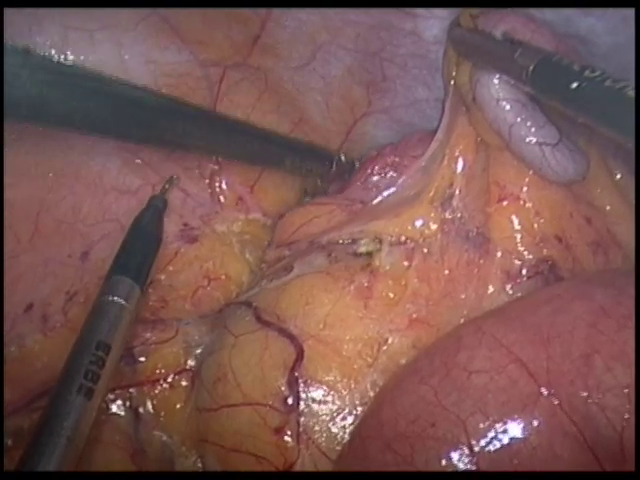
\includegraphics[width=0.8\linewidth]{sfb_original}
    	\caption{An example image from the medical dataset. Image from TODO: cite.}
    	\label{fig:sfb_original}
	\end{subfigure}
	\hfill
	\begin{subfigure}[t]{0.47\textwidth}
	\centering
    	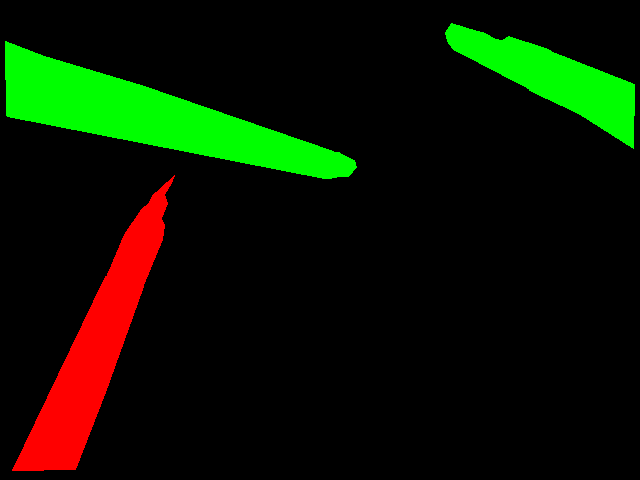
\includegraphics[width=0.8\linewidth]{sfb_segmentation}
    	\caption{The corresponding segmentation mask to the image in fig \ref{fig:sfb_original}. The colors encode the tools' classes. Taken from TODO: cite.}
    	\label{fig:sfb_segmentation}
	\end{subfigure}
	\caption{An example image and its corresponding segmentation mask from the medical dataset.}
	\label{fig:sfb}
\end{figure} 

\section{Medical Images}

The goal of this work is to provide a system to successfully and efficiently annotate the medical images that were provided upfront. The dataset includes segmentation masks but no object models or existing pose annotations. An example image together with the corresponding segmentation mask are given in \fig \ref{fig:sfb}. The dataset resembles the characteristics and quality of images from laparoscopic videos, i.e. there is no depth information present and occlusion and artifacts like motion blur can occur. The issues with this dataset are discussed in section \ref{section:6dpat_difficulties}. 

\section{6D Pose Annotation Tool (6D-PAT)}

\begin{figure}[!tbp]
	\centering
	\begin{subfigure}[t]{0.47\textwidth}
		\centering
    	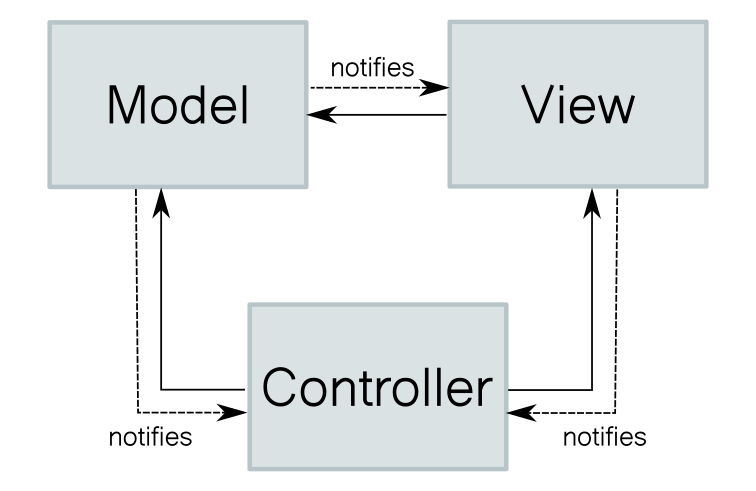
\includegraphics[width=0.8\linewidth]{mvc}
    	\caption{The Model-View-Controller architecture. The solid lines stand for a direct connection either because the target is owned or known by reference. The dashed line is an indirect connection using for example the observer pattern or the Qt Signals and Slots mechanism visible in \fig \ref{fig:qt_signals_slots}. Own image.}
    	\label{fig:mvc}
	\end{subfigure}
	\hfill
	\begin{subfigure}[t]{0.47\textwidth}
	\centering
    	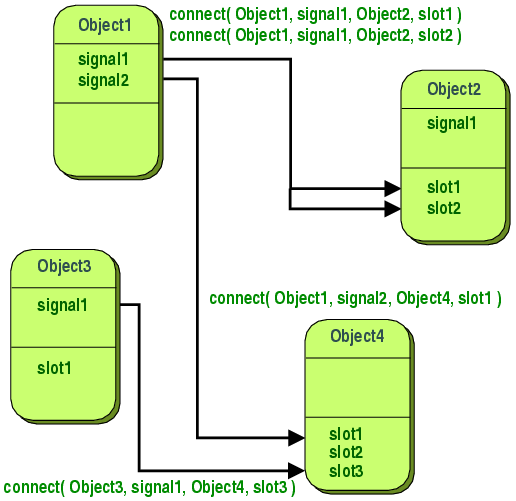
\includegraphics[width=0.8\linewidth]{qt_signals_slots}
    	\caption{The Signals and Slots mechanism of Qt. A class can define signals it can emit, independently of any listeners waiting for that signal. Slots are the functions that, when connected a signal, are called and can thus react to the signal. Image from \cite{qt_signals_and_slots}.}
    	\label{fig:qt_signals_slots}
	\end{subfigure}
	\caption{Two basic architectural concepts used in \gls{6dpat}: the model view controller pattern and the signal and slots pattern.}
\end{figure} 

The creation of sufficient training data for neural networks can be a time-consuming and tedious process. Using non-specialized tools designed for other purposes, like 3D modeling programs, require the personnel creating the annotations to get accustomed to complex user interfaces (\gls{ui}s). The goal of the annotation tool is to provide a system that allows easy and efficient annotation of images, images of the medical dataset in particular. The annotated poses, the so-called \textit{Ground-Truth Poses} (see section \ref{section:terminology}), can later be used to train a neural network. The program is written in the language C++ and named \textit{6D - Pose Annotation Tool (\gls{6dpat})}. Its logo can be seen in \fig \ref{fig:6dpat_logo}. Although the program was developed using the \textit{Linux}-based operating system \textit{Ubuntu}, it is compilable on other systems as well.

\subsection{Frameworks \& Third-Party Libraries}

The listed frameworks are all necessary dependencies of the annotation tool. There are no dependencies other than the mentioned ones. They are not part of the repository but have to be compiled individually instead. Since all three frameworks/libraries are platform-independent the program can be compiled and run on different systems. \\

\noindent\textbf{Qt.} \textit{Qt} \cite{qt} is a powerful framework for C++ that offers a vast selection of user interface components but also general functionality that exceeds the capabilities of the standard C++ library. Qt is also chosen as the main framework because it ensures portability of C++ applications by encapsulating system calls of all kind. The program \textit{Qt Creator} is the \textit{Integrated Development Environment (IDE)} that is included in the Qt distribution was used to write and execute the code of \gls{6dpat}. An IDE combines an editor to edit code an some environment to execute it. \\

\noindent\textbf{OpenGL.} \textit{OpenGL} \cite{opengl} is a widespread open-source 3D graphics library specification. Implementations for many operating systems exist, thus making most OpenGL using applications compilable in different environments without further modifications. \textit{Mesa 3D} \\

\noindent\textbf{OpenCV.} \textit{OpenCV} \cite{opencv} is a C++ library created for various computer vision tasks, hence the name. OpenCV provides implementations for tracking, object detection, segmentation and many more. In this work its \textit{solvePnPRansac} is used. \\

\begin{figure}[!tbp]
	\centering
    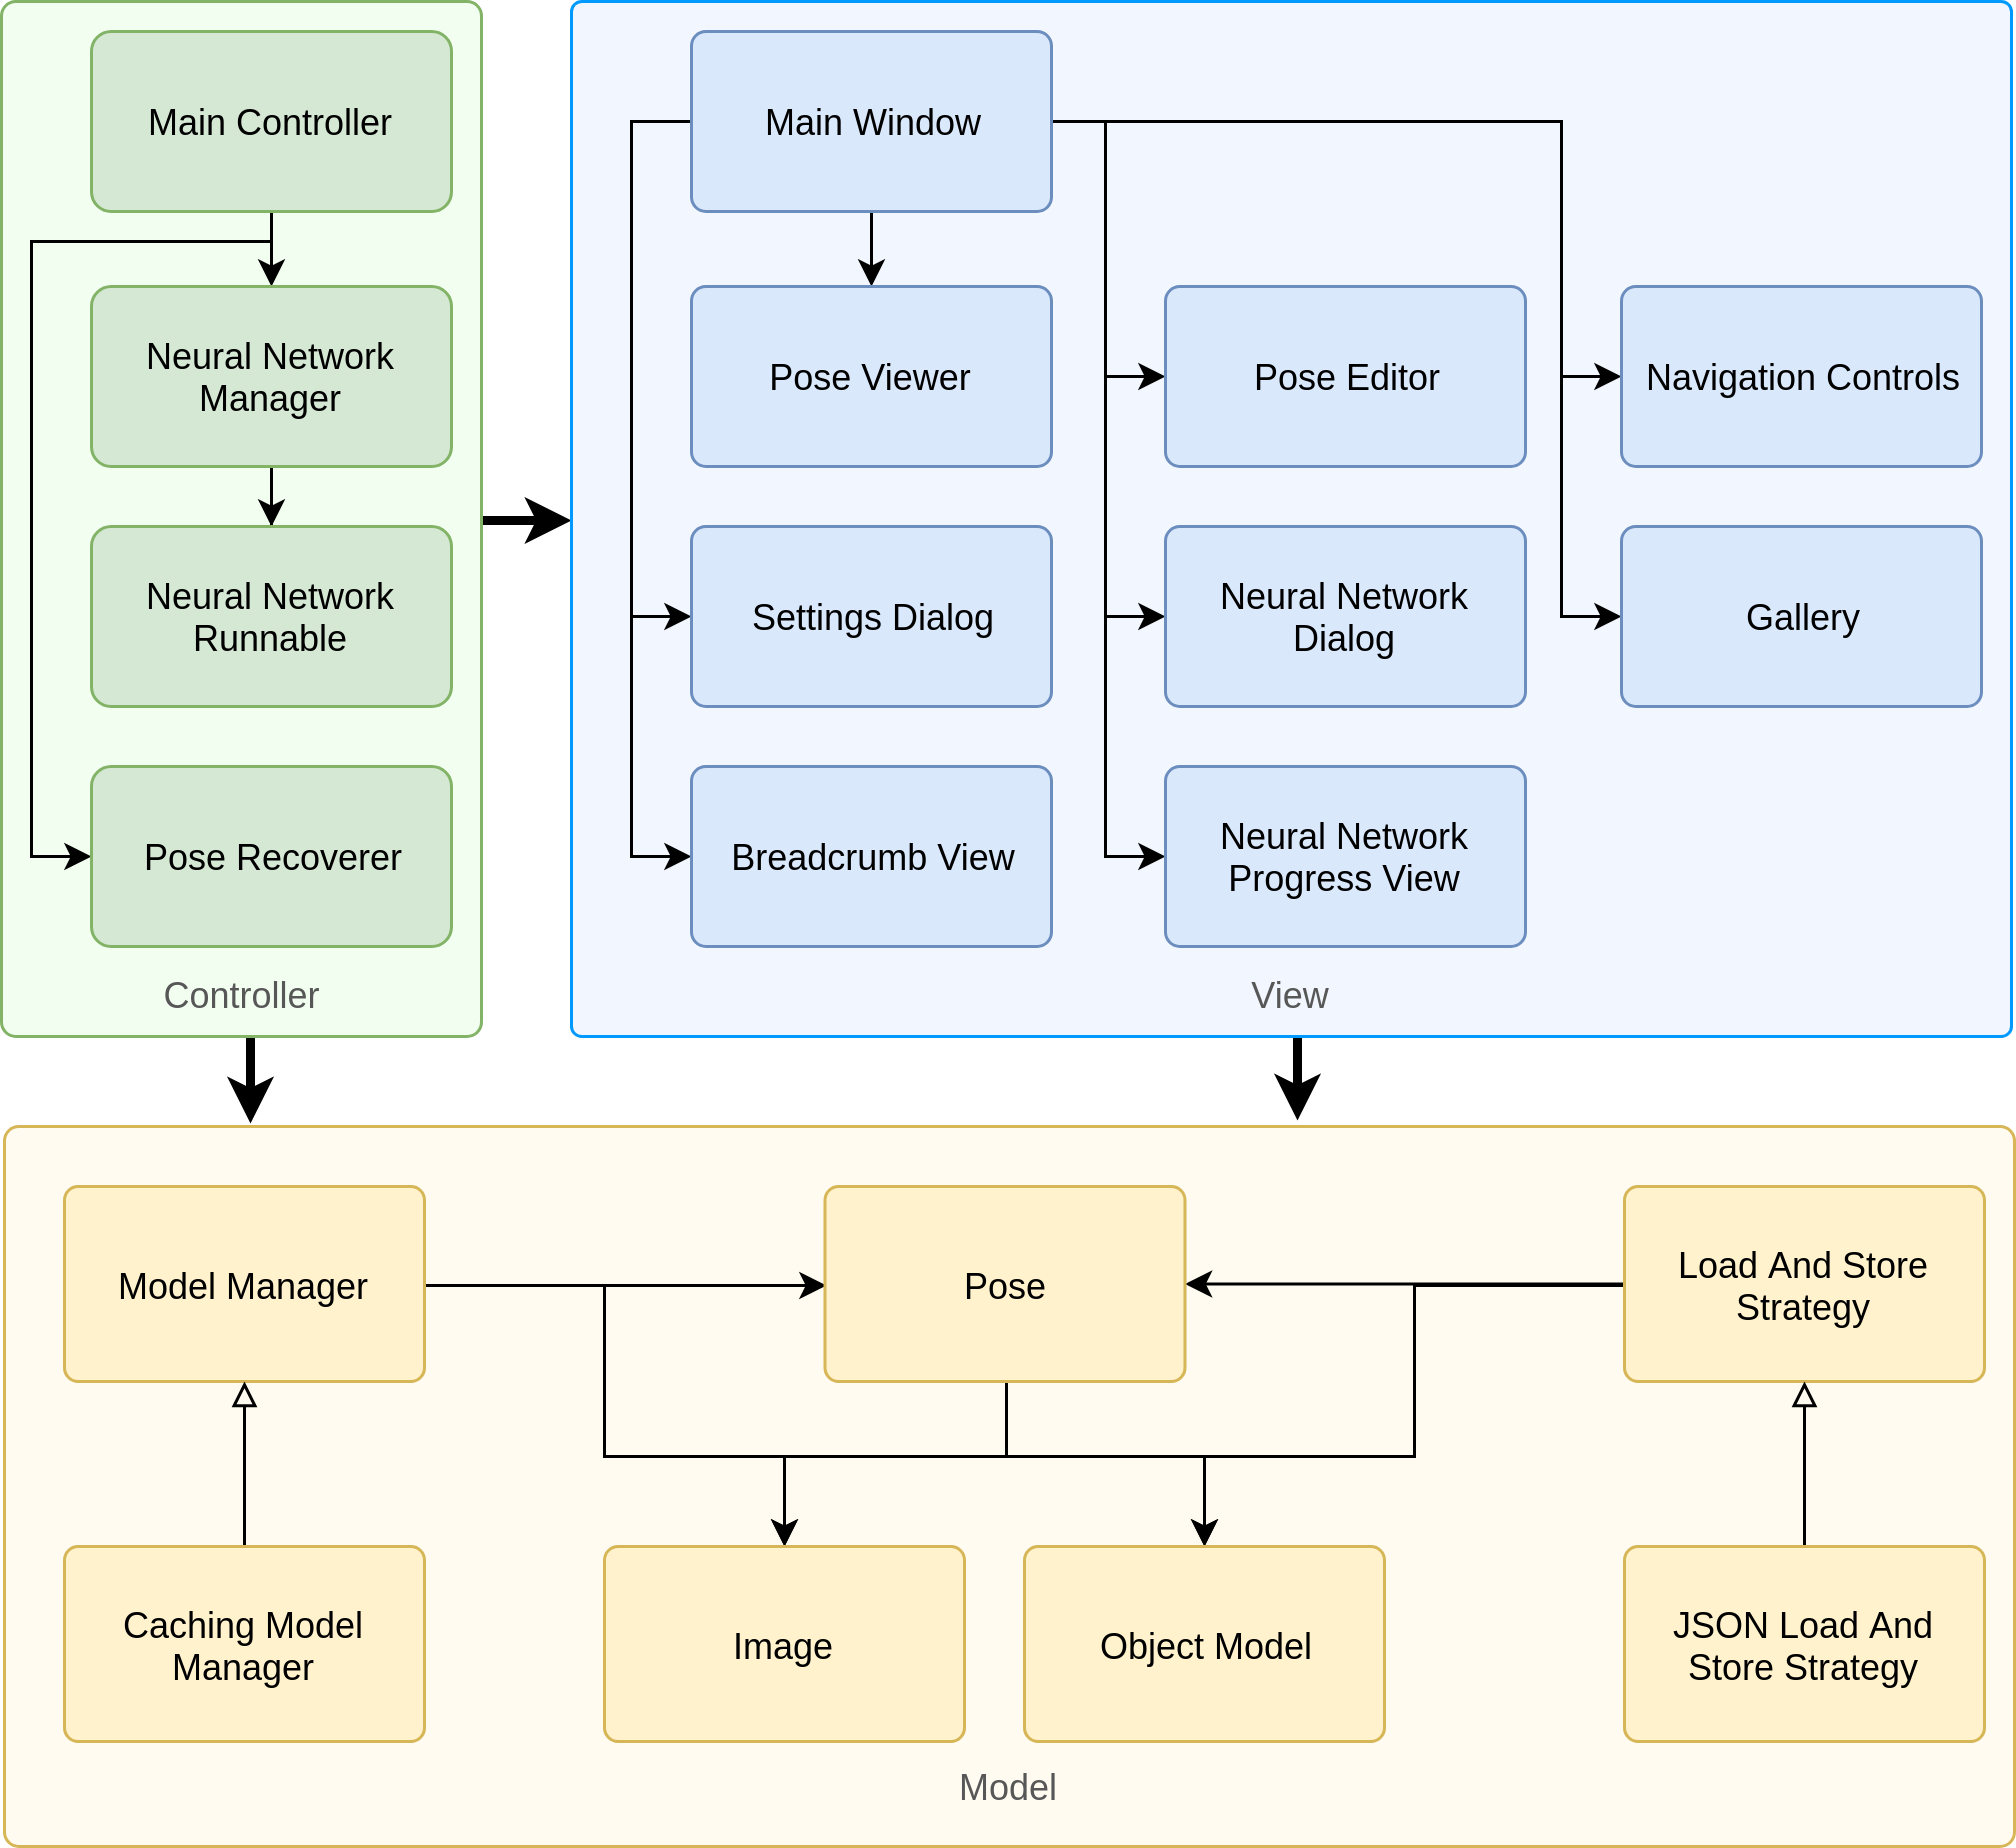
\includegraphics[width=0.9\linewidth]{6dpat_class_diagram}
    \caption{An abstract high-level class diagram of the a subset of the classes of \gls{6dpat}. The thin filled-out arrow-heads mean "uses". The not filled arrow head mean "inherits". Arrows pointing from the larger rectangles imply that the source rectangle uses classes of the target rectangle, although not all classes use all target classes. The \textbf{Main Controller} holds the references to the \textbf{Pose Creator}, the \textbf{Neural Network Manger} and the \textbf{Neural Network Runnable}. The Pose Creator stores the clicked 2D-3D correspondences and implements functionality to recover a pose. The Neural Network Manager controls the connection to the neural network and uses the Neural Network Runnable to execute network tasks. The Main Controller also owns the \textbf{Main Window}, which consists mainly of the classes visible in the "View" rectangle. The \textbf{Pose Viewer} can display images and their poses and the \textbf{Pose Editor} can be used to edit those poses. The \textbf{Settings Dialog} allows editing of several preferences. To let the network predict poses, the user can open the \textbf{Neural Network Dialog} and select images to run prediction on. This opens the \textbf{Neural Network Progress View} until inference has finished. The \textbf{Breadcrumb View} shows the currently set folders to load images and object models from. The \textbf{Navigation Controls} allow navigation through the \textbf{Galleries} showing the images and object models. The \textbf{Model Manager} uses the \textbf{Load And Store Strategy} to load images, object models and poses. The respective classes are depicted in the middle of the large rectangle labeled "Model". The Main Controller owns the Model Manager and passes it to most view classes. Own image.}
    \label{fig:6dpat_class_diagram}
\end{figure} 

\noindent\textbf{Assimp.} \textit{Assimp} \cite{assimp} is a C++ library designed to import 3D models. The library was incorporated into the tool to ensure a broad support of 3D model formats.

\subsection{Architecture \& Code Design}

\gls{6dpat} is primarily a \textit{Graphical User Interface (GUI)} program, i.e. its purpose is to display a window and enable optical interaction like clicking. Thus, the chosen underlying architecture is \textit{Model-View-Controller (\gls{mvc})}, which separates the concerns of data management (Model), displaying data (View) and high level logic (Controller). The schematic of the \gls{mvc} architecture is given in \fig \ref{fig:mvc}. The indirect connections are realized via the Qt Signals and Slots mechanism, which is visualized in \fig \ref{fig:qt_signals_slots}. To speed up interface creation, \textit{Qt Designer} was used to layout the views. Qt Designer is a graphical tool that allows placement of UI components and linking of signals and slots. \\

The most important C++ classes of the program are displayed in \fig \ref{fig:6dpat_class_diagram}. The diagram is simplified for easier understanding. The arrows from the large rectangles imply usage of the classes in the target rectangle. This does not necessarily mean, that all classes of the source use all classes of the target rectangle. The \textit{Pose Editor} uses the \textit{Model Manager} but the \textit{Breadcrumb View} does not, for example. The general structure of the program is the following: the main controller holds references to the \textit{Neural Network Manager}, the \textit{Pose Creator} and the \textit{Main Window}. The neural network manager uses the \textit{Neural Network Runnable} the execute training and inference tasks with the neural network. The pose creator manages the currently clicked corresponding points and computes the new pose when requested and enough corresponding points were clicked. The main window consists of the two main widgets \textit{Pose Editor} and \textit{Pose Viewer}. The pose editor can display an object model $O$ selected from the objects gallery and allows editing all poses $P$ of an image $I$ selected from the images gallery. Both \textit{Gallerys} are owned by the main window, as well. The pose viewer in turn renders all poses $P$ of an image $I$ onto the image. Pose viewer and editor can be used to create new poses (see section \ref{subsection:correspondence_and_pose_creation}). The main window also dispalys the paths selected to load images and object models from using the \textit{Breadcrumb Views}, and allows navigation through the gallerys via the \textit{Navigation Controls}. The settings dialog can be opened from the to edit the preferences of the program. To run the network inference ,the \textit{Neural Network Dialog}, owned by the main window, can be openend to select the images to run prediction on. The main window then displays the \textit{Neural Network Progress View}. Most view classes use the model manager, the \textit{Pose}, the \textit{Object Model} and the \textit{Image} class. Their use should be clear. The main controller sets the \textit{Load And Store Strategy} on the model manager. This class is responsible for reading imags and object models from the hard-drive, as well as persiting poses. The \textit{JSON Load And Store Strategy} uses the JSON format to store poses and read camera matrices. The \textit{Caching Model Manager} is a simple implementation of the model manager interface that chaches images, object models and poses instead of delegating all loading calls to the strategy.

The program expects the camera information and the ground-truth poses file to be in \textit{JSON format}. JSON is a format that is relatively easy for humans to read and is used by many deep learning applications. Transforming JSON formats can be done quickly and therefore provides the possibility to read data from other projects. \\

The program offers functionality to start the network inference. We realized this feature by starting a new process. It is not necessary to use the official C++ Python bridge, offered by the maintainers of Python. The network writes the inferred poses back to a JSON file and we do not need to retrieve any return values directly.

\subsection{Manual Annotation} 

This sections describe the user interface of \gls{6dpat} and the required steps to annotate images with 6D poses. The process needs some actions performed before the actual annotation can be begin. 

\subsubsection{Preparation}

\begin{figure}[!tbp]
	\centering
	\begin{subfigure}[t]{\textwidth}
		\centering
    	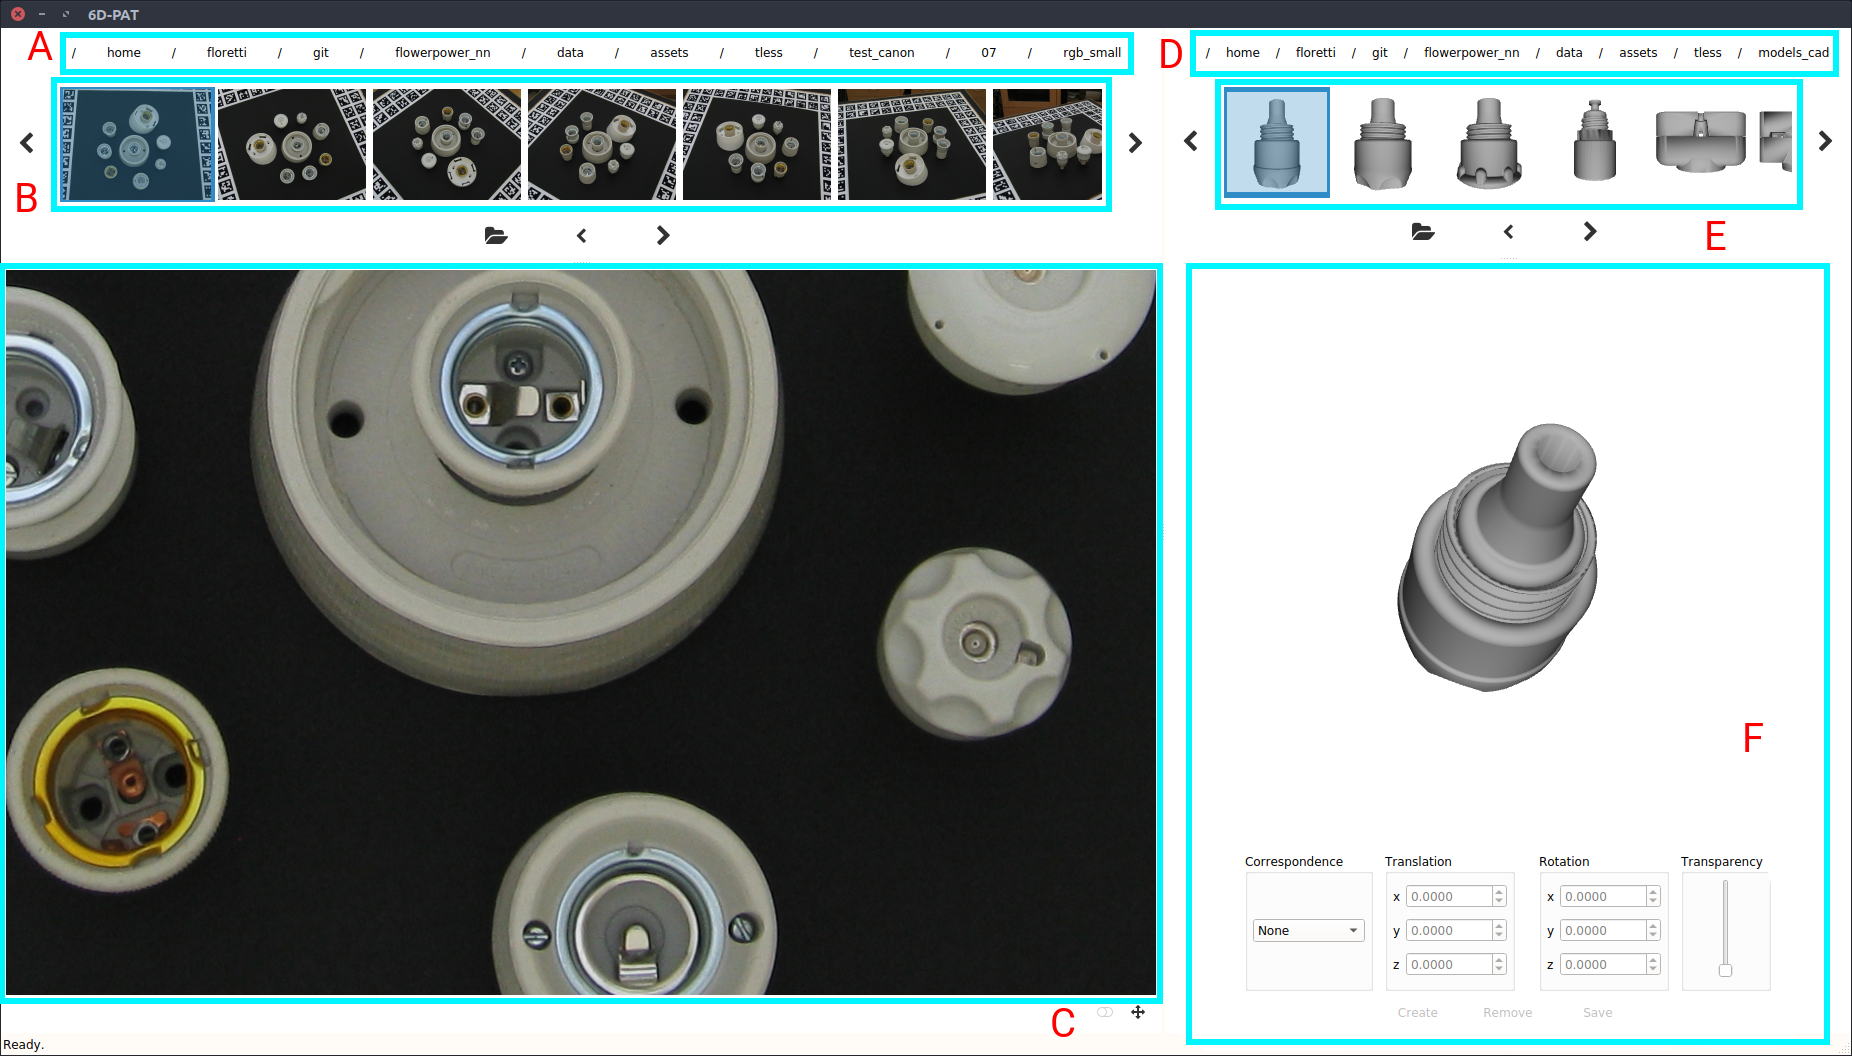
\includegraphics[width=\linewidth]{6dpat_components}
    	\caption{The user interface of the annotation tool \gls{6dpat}. The data displayed are images and object models from the T-Less dataset. The components marked with a turquoise box are the following ones: \textbf{A}: The full path of the currently selected folder to load images from. \textbf{B}: The gallery showing the images loaded from the selected path. \textbf{C}: The \textit{Pose Viewer} shows the image selected in gallery B. The user can click on the image to define the 2D point of a new pose. \textbf{D}: The full path of the currently selected folder to load object models from. \textbf{E}: The rendered 3D preview of the object models loaded from the selected path. \textbf{F}: The \textit{Pose Editor} shows the object model selected in gallery E. The user can click on the object model to complete the correspondence with the 3D point. the controls at the bottom can be used to edit existing poses. Own image.}
    	\label{fig:6dpat_components}
	\end{subfigure}
	\par\bigskip
	\begin{subfigure}[t]{0.47\textwidth}
		\centering
    	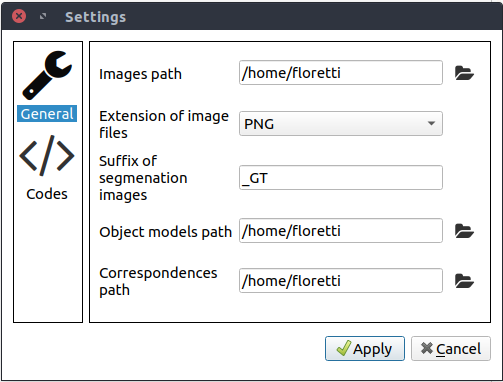
\includegraphics[width=0.8\linewidth]{6dpat_settings}
    	\caption{The settings dialog of \gls{6dpat}. From here the paths to the images and object models can be set, as well as the segmentation image suffix the image type and the file to write the poses to. Own image.}
    	\label{fig:6dpat_settings}
	\end{subfigure}
	\hfill
	\begin{subfigure}[t]{0.47\textwidth}
	\centering
    	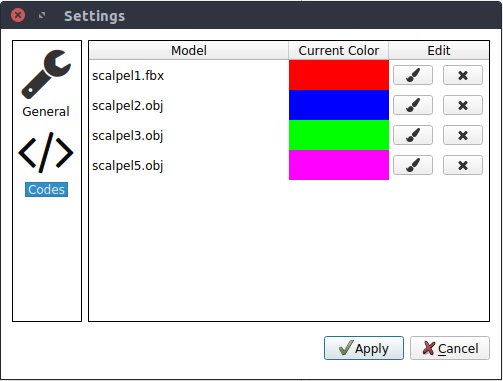
\includegraphics[width=0.8\linewidth]{6dpat_settings_codes}
    	\caption{The settings dialog while editing the colors of the object models in the segmentation images. Own image.}
    	\label{fig:6dpat_settings_codes}
	\end{subfigure}
	\caption{The main view of \gls{6dpat} as well as the two settings views.}
	\label{fig:6dpat_ui_overview}
\end{figure}

The first step after starting the program is to open the settings (see \fig \ref{fig:6dpat_settings}) and set the path to the images that are to be annotated, as well as the path to the folder that contains the object models that should be used for annotation. 

The folder of the images has to contain a JSON file that holds the camera matrix $K$ for each individual image. If no camera info file exists, a Python script, that is distributed with the neural network, can be used to created approximate camera matrices. The path to the segmentation images (if any) has to be set as well. The program loads the images and the segmentation images and sorts them by the numbers in their filenames and then matches image $I$ at index $j$ with the segmentation image $S$ at index $j$. 

Lastly, the location of the JSON file where the ground-truth poses are to be written to has to be specified. If no such file exists an empty one can be created and selected. If segmentation images are present they are linked to the respective image and can be viewed by activating the toggle at the bottom right corner of the pose viewer (the program displaying a segmentation image can be seen in \fig \ref{fig:sfb_segmentation}). 

If required, the colors of the object models in the segmentation images can be set using the settings dialog as shown in \fig \ref{fig:6dpat_settings_codes}. This can reduce the number of displayed tools if many different tools are needed for annotation.

\subsubsection{Correspondence and Pose Creation} \label{subsection:correspondence_and_pose_creation}

The association of letter and component of the annotation tool are visualized in \fig \ref{fig:6dpat_components}. To annotate a new pose an image $I$ has to be selected from gallery \textit{B}, first. The pose viewer \textit{C} then displays the image. The model $O$ that the image is to be annotated with can be selected from the gallery \textit{E}. The pose editor \textit{F} shows the selected object model. The user can rotate the object the reach otherwise hidden areas of it. The arrow keys can be used to move the object along the $x$ and $y$ and also, if the shift key is pressed, along the $z$ axis. 

When the object is in an appropriate position, the user can begin to create a correspondence $C$ by clicking on $I$ and this way defining the 2D point $u$ of the correspondence. To complete the correspondence, the object model $O$ has to be clicked at the respective position $p$. This procedure has to be repeated until enough correspondences have been defined to create the new pose $P$. The minimum is 4 correspondences. 

The creation process is shown in \fig \ref{fig:6dpat_correspondence_creation}. More correspondences can make the initial pose more accurate. Clicking the "Create" button at the bottom of the pose viewer creates the pose $P$ using the correspondences $C_i$ and OpenCV's \textit{solvePnPRansac} method. The newly created pose is directly selected for editing and can be refined using the controls of the pose viewer. After pose refinement it is necessary to click the "Save" button. 

The slider labeled "Transparency" can be used to reduce the object's opacity on the image. After all poses have been annotated successfully the next image can be selected from the gallery B. This operation has to be repeated until the dataset is fully annotated, although intermediate states can be used to train the network already (see chapter \ref{chapter:semi_automatic}).

It is possible to use the neural network to predict poses. This requires a proper setup and training of the network beforehand. The prediction process can be started by clicking the "Predict" button in the lower right corner of the pose editor.

\begin{figure}[!tbp]
	\centering
    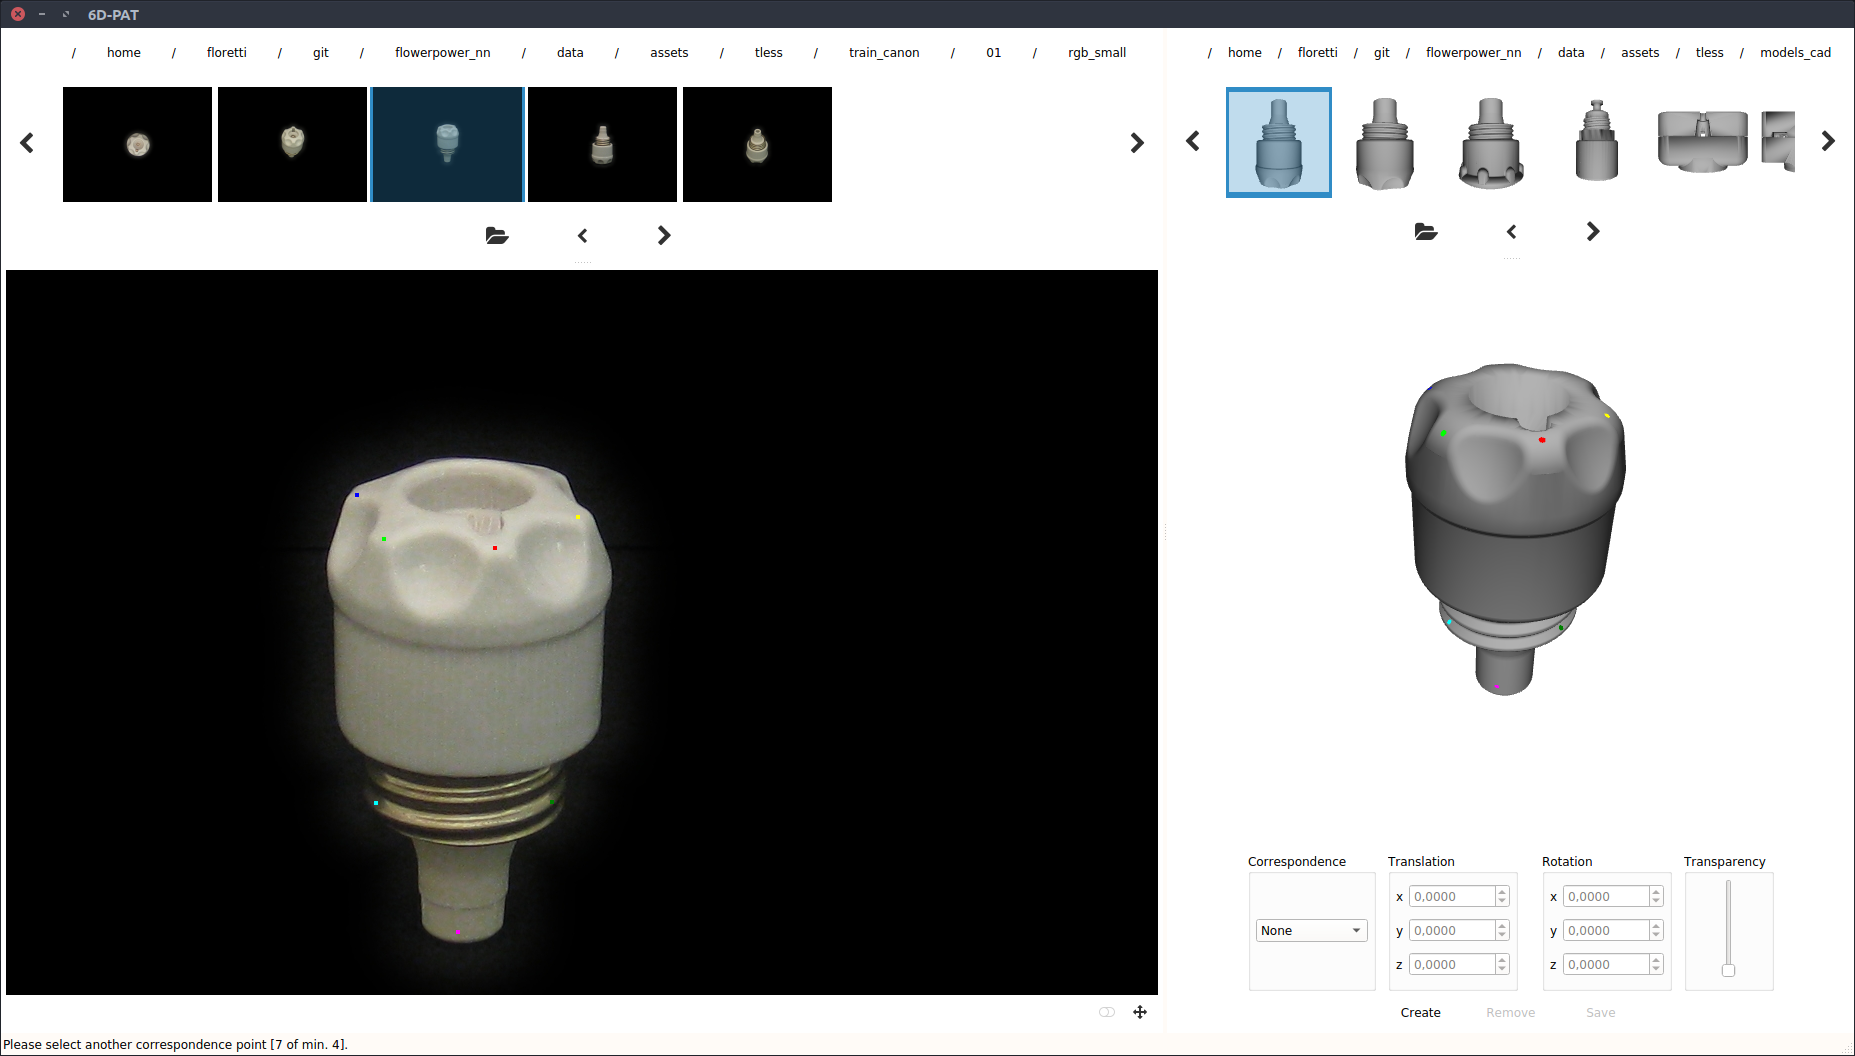
\includegraphics[width=\linewidth]{6dpat_correspondence_creation}
    \caption{The pose creation process. The user has to click the image first and then the corresponding 3D location on the object model. The red circles and red lines were added afterwards to emphasize the colored dots which the program draws. Own image.}
    \label{fig:6dpat_correspondence_creation}
\end{figure} 

\subsection{Problems \& Difficulties} \label{section:6dpat_difficulties}

\begin{figure}[!tbp]
	\begin{subfigure}[t]{0.47\textwidth}
		\centering
    	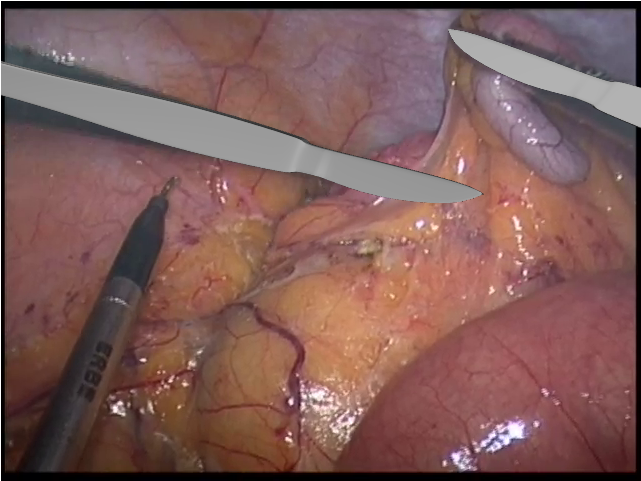
\includegraphics[width=\linewidth]{6dpat_sfb_image}
    	\caption{An image from the medical images dataset annotated using 6D-PAT. The correct rotation and translation are difficult to estimate without the actually used tools. Own image.}
    	\label{fig:6dpat_sfb_image}
	\end{subfigure} 
	\hfill
	\begin{subfigure}[t]{0.47\textwidth}
		\centering
    	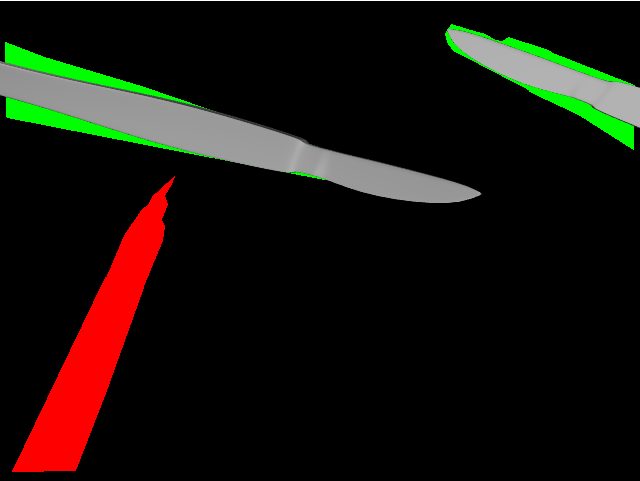
\includegraphics[width=\linewidth]{6dpat_sfb_segmentation}
    	\caption{The corresponding segmentation image to the image on the right. The discrepancy between the segmentation masks and the object model is clearly visible as the green area. Own image.}
    	\label{fig:6dpat_sfb_segmentation}
	\end{subfigure} 
\end{figure} 

During the implementation of the program multiple problems arose and complicated the development process. The most drastic ones are mentioned in this section. Issues contradicting the initial usage patterns and their impact on the final design of the program are explained, as well. \\

One of the major factors that prolong the implementation process was the usage of the only recently released \textit{Qt3D}, which is part of the Qt framework. Qt3D's purpose is to encapsulate graphics programming to increase portability of applications including 3D graphics. The incomplete documentation and unintuitive concepts make it difficult to use without consultation. After more and more complications emerged in the almost completed product the Qt3D framework was deemed unusable and omitted in favor of a native OpenGL implementation. \\

Initially, a desired feature of the program was to present a next unannotated image when the user annotated all poses of an image. This is not feasible for multiple reasons. First of all, a user might still not be content with the poses and might signal that they are finished with the annotation process too early. Thus, it might be disturbing when the program automatically shows the next image. 

The datasets to annotate can also have very distinct characteristics, which require the user to choose the next image personally. For a dataset like T-Less, many images have to be skipped due to their similarity. Intuitively, the more diverse poses are annotated, the better a neural network can be trained. Instead of forcing the user to annotate varying images the motivation should be the sped up annotation process as soon as the neural network is able to make plausible predictions. 

The diversity of kinds of dataset is also the reason why the program does not provide functionality to initialize the next poses based on the ones in the last image. This feature would imply too many assumptions on the dataset and, in the worst case, cause more work for the user. \\

While trying to annotate the medical images dataset it became clear, that proper 3D models are crucial for successful annotation. To temporarily annotate the medical images, 3D surgical tools were downloaded from the internet as a replacement for the missing object models. But having a different shape and also missing the distinctive features of the real objects makes in very difficult to estimate the ground-truth pose. 

The influence of contradicting annotated poses during training of a network is not clear. The author of this work strongly recommends to obtain the correct 3D models before annotating the medical images. The issue of the object models not fitting the segmentation mask can be seen in \fig \ref{fig:sfb_segmentation}. \fig \ref{fig:sfb_original} shows the actual image and the discrepancy between the models and the pixels belonging to the models.

A first try to use the official Python bindings did not work to our complete satisfaction. The rather involved alterations to the program to be able to handle the Python script running inference are too complex compared to starting an external process. Qt offers this functionality already.

The Python binding is not complete yet. Training is not possible and the a deep learning expert has to setup the network and its parameters to enable its usage in the program. The current state of the incorporation of the network is to be seen as a proof of concept that requires further development.

Because the neural network is trained only for one object, the time-intensive step (proportional to the overall time needed for inference on one image) of loading the trained weights has to be performed each time when running inference for different objects. The frame of this work was to explore neural networks trained for one object only.

%%%%%%%%%%% TODO: Evaluation














% Time per annotation etc

T-Less Test images:

0000.jpg 2:30min

0150.jpg 1:23min

0250.jpg: 2:05min

0350.jpg: 3:06min

0500.jpg: 0:50min












%%%%%%%%%%% TODO: Evaluation

\subsection{Future Improvements of \gls{6dpat}}

To provide an outlook how the program can be improved in the future, some key problems as well as their solutions are mentioned here. An important feature that should be implemented is moving the object models around on the displayed image by dragging them. It should also be possible to rotate them with the mouse. The initial poses of the models using the clicking procedure are pretty accurate in many cases already. But sometimes, when the camera is looking along an axis of the object directly, it happens that the rotation is far off. The user can correct the poses with the provided controls. But using them takes some skill and time. The described editing process would profit in terms of time needed per annotation. To give the user a better overview over the image and its annotated poses, a zoom option should be implemented, as well.

The problem of the time needed for loading the weights of the neural network could be solved by offering an intermediate screen that allows to select many images and the object that is to be annotated. The time of loading the weights gets amortized when running inference for many images. 

Another suggested step is to fully incorporate the network in the annotation tool. This way inexperienced users can profit from the network without the need for an expert every time they want it to detect poses in an image. There is probably no way to automatize setting up the network as this requires knowledge of neural nets. In an ideal setting it can be kept to a minimum and users can be introduced to the most relevant parameters, which they can set from within the program.